\begin{frame}
  \frametitle{The Rescorla-Wagner equations}
  %% \framesubtitle{}

  \begin{itemize}
  \item<1-> Goal of naïve discriminative learner: predict an \primary{outcome} $O$ based on presence or absence of a set of \primary{cues} $C_1, \ldots, C_n$
  \item<2-> An \primary{event} $(\vc, o)$ is formally described by indicator variables
    \begin{align*}
      c_i &= 
       \begin{cases}
         1 & \text{if $C_i$ is present} \\
         0 & \text{otherwise}
       \end{cases}
      &
      o &= 
       \begin{cases}
         1 & \text{if $O$ results} \\
         0 & \text{otherwise}
       \end{cases}
    \end{align*}
  \item<3-> Given cue-outcome \primary{associations} $\vv = (V_1, \ldots, V_n)$ of learner, the \primary{activation level} of the outcome $O$ is
    \[
    \only<beamer:3| handout:1>{
      \sum_{j=1}^n c_j V_j}
    \only<beamer:4-| handout:0>{
      \sum_{j=1}^n c_j\psupt V_j\psupt}
    \]
  \item<4-> Associations $\vv[t]$ as well as cue and outcome indicators $(\vc[t], o\psupt)$ depend on time step $t$
  \end{itemize}
\end{frame}

\begin{frame}
  \frametitle{The Rescorla-Wagner equations}
  %% \framesubtitle{}
  
  \begin{itemize}
  \item \citet{Rescorla:Wagner:72} proposed the \primary{R-W equations} for the change in associations given an event $(\vc, o)$:
    \[
    \Delta V_i =
    \begin{cases}
      0 & \text{if } c_i = 0\\
      \alpha_i \beta_1 \bigl(\lambda - \sum_{j=1}^n c_j V_j \bigr) & \text{if } c_i = 1 \wedge o = 1 \\
      \alpha_i \beta_2 \bigl(0 - \sum_{j=1}^n c_j V_j \bigr) & \text{if } c_i = 1 \wedge o = 0 
    \end{cases}
    \]
    with parameters
    \ungap[.5]
    \begin{align*}
      \lambda &> 0   && \text{target activation level for outcome $O$} \\
      \alpha_i &> 0  && \text{salience of cue $C_i$} \\
      \beta_1 &> 0   && \text{learning rate for positive ovents ($o = 1$)} \\
      \beta_2 &> 0   && \text{learning rate for negative ovents ($o = 0$)}
    \end{align*}
  \end{itemize}
\end{frame}

\begin{frame}<beamer:1-3| handout:1>
  \frametitle{The Widrow-Hoff rule}
  %% \framesubtitle{}
  
  \begin{itemize}
  \item The \primary{W-H rule} \citep{Widrow:Hoff:60} is a widely-used simplification of the R-W equations:
    \begin{align*}
    \Delta V_i &=
    \begin{cases}
      0 & \text{if } c_i = 0\\
      \only<beamer:1| handout:0>{\alpha_i} \beta\only<beamer:1| handout:0>{_1} \bigl(\only<beamer:1| handout:0>{\lambda}\only<beamer:2-| handout:1>{1} - \sum_{j=1}^n c_j V_j \bigr) & \text{if } c_i = 1 \wedge o = 1 \\
      \only<beamer:1| handout:0>{\alpha_i} \beta\only<beamer:1| handout:0>{_2} \bigl(0 - \sum_{j=1}^n c_j V_j \bigr) & \text{if } c_i = 1 \wedge o = 0 
    \end{cases}
    \only<beamer:3-| handout:1>{\\
       &= \primary{c_i \beta \bigl( o - \textstyle\sum_{j=1}^n c_j V_j \bigr)}}
    \end{align*}
    with parameters
    \ungap[.5]
    \begin{align*}
      \lambda  &= 1   && \text{target activation level for outcome $O$} \\
      \alpha_i &= 1  && \text{salience of cue $C_i$} \\
      \beta_1  &= \beta_2   && \text{global learning rate for positive and}\\
               &= \beta > 0 && \text{negative events}
    \end{align*}
  \end{itemize}
\end{frame}

\begin{frame}[c]
  \frametitle{A simple example: German noun plurals}
  %% \framesubtitle{}
  
  \small\centering
  \begin{tabular}{r>{\color{counterpoint}}l|c|cccccc}
    \toprule
    $t$ & & $o$ & $c_1$ & $c_2$ & $c_3$ & $c_4$ & $c_5$ & $c_6$ \\
    & \secondary{word} & \secondary{pl?} & \secondary{\emph{--e}} & \secondary{\emph{--n}} & \secondary{\emph{--s}} & \secondary{umlaut} & \secondary{dbl cons} & \secondary{bgrd}\\
    \midrule
    1 &   Bäume &  1  &  1 & 0 & 0 & 1 & 0 & 1 \\ 
    2 & Flasche &  0  &  1 & 0 & 0 & 0 & 0 & 1 \\ 
    3 &    Baum &  0  &  0 & 0 & 0 & 0 & 0 & 1 \\ 
    4 &  Gläser &  1  &  0 & 0 & 0 & 1 & 0 & 1 \\ 
    5 &Flaschen &  1  &  0 & 1 & 0 & 0 & 0 & 1 \\ 
    6 &   Latte &  0  &  1 & 0 & 0 & 0 & 1 & 1 \\ 
    7 &  Hütten &  1  &  0 & 1 & 0 & 1 & 1 & 1 \\ 
    8 &    Glas &  0  &  0 & 0 & 1 & 0 & 0 & 1 \\ 
    9 &   Bäume &  1  &  1 & 0 & 0 & 1 & 0 & 1 \\ 
   10 &    Füße &  1  &  1 & 0 & 0 & 1 & 0 & 1 \\
    \bottomrule
  \end{tabular}
\end{frame}

\begin{frame}[c]
  \frametitle{A simple example: German noun plurals}
  %% \framesubtitle{}
  
  \footnotesize\centering
  \begin{tabular}{>{\color{counterpoint}}c|c|cccccc}
    \toprule
    \secondary{$t$} & \secondary{$\sum c_j V_j$} & \secondary{$V_1$} & \secondary{$V_2$} & \secondary{$V_3$} & \secondary{$V_4$} & \secondary{$V_5$} & \secondary{$V_6$} \\
\only<beamer:1| handout:0>{\color{foreground}  1 & .000 & .000 & .000 &  .000 & .000 &  .000 & .000 }% 
\only<beamer:2| handout:0>{\color{foreground}  2 & .400 & .200 & .000 &  .000 & .200 &  .000 & .200 }% 
\only<beamer:3| handout:0>{\color{foreground}  3 & .120 & .120 & .000 &  .000 & .200 &  .000 & .120 }% 
\only<beamer:4| handout:0>{\color{foreground}  4 & .296 & .120 & .000 &  .000 & .200 &  .000 & .096 }% 
\only<beamer:5| handout:0>{\color{foreground}  5 & .237 & .120 & .000 &  .000 & .341 &  .000 & .237 }% 
\only<beamer:6| handout:0>{\color{foreground}  6 & .509 & .120 & .153 &  .000 & .341 &  .000 & .389 }% 
\only<beamer:7| handout:0>{\color{foreground}  7 & .679 & .018 & .153 &  .000 & .341 & -.102 & .288 }% 
\only<beamer:8| handout:0>{\color{foreground}  8 & .352 & .018 & .217 &  .000 & .405 & -.038 & .352 }% 
\only<beamer:9| handout:0>{\color{foreground}  9 & .704 & .018 & .217 & -.070 & .405 & -.038 & .281 }% 
\only<beamer:10| handout:1>{\color{foreground}10 & .882 & .077 & .217 & -.070 & .464 & -.038 & .340 }% 
\only<beamer:11| handout:0>{\color{foreground}11 &      & .101 & .217 & -.070 & .488 & -.038 & .364 }%
    \\
    \midrule
    \only<beamer:1| handout:0>{   Bäume &  1  &  1 & 0 & 0 & 1 & 0 & 1 \\ }% 
    \only<beamer:2| handout:0>{ Flasche &  0  &  1 & 0 & 0 & 0 & 0 & 1 \\ }% 
    \only<beamer:3| handout:0>{    Baum &  0  &  0 & 0 & 0 & 0 & 0 & 1 \\ }% 
    \only<beamer:4| handout:0>{  Gläser &  1  &  0 & 0 & 0 & 1 & 0 & 1 \\ }% 
    \only<beamer:5| handout:0>{Flaschen &  1  &  0 & 1 & 0 & 0 & 0 & 1 \\ }% 
    \only<beamer:6| handout:0>{   Latte &  0  &  1 & 0 & 0 & 0 & 1 & 1 \\ }% 
    \only<beamer:7| handout:0>{  Hütten &  1  &  0 & 1 & 0 & 1 & 1 & 1 \\ }% 
    \only<beamer:8| handout:0>{    Glas &  0  &  0 & 0 & 1 & 0 & 0 & 1 \\ }% 
    \only<beamer:9| handout:0>{   Bäume &  1  &  1 & 0 & 0 & 1 & 0 & 1 \\ }% 
    \only<beamer:10| handout:1>{   Füße &  1  &  1 & 0 & 0 & 1 & 0 & 1 \\}% 
    \only<beamer:11| handout:0>{& & & & & & & \\ }%
    \phantom{Flaschen} & \secondary{$o$} & \secondary{$c_1$} & \secondary{$c_2$} & \secondary{$c_3$} & \secondary{$c_4$} & \secondary{$c_5$} & \secondary{$c_6$} \\
    \bottomrule
  \end{tabular}

  \gap[1]
  \only<beamer:1| handout:0>{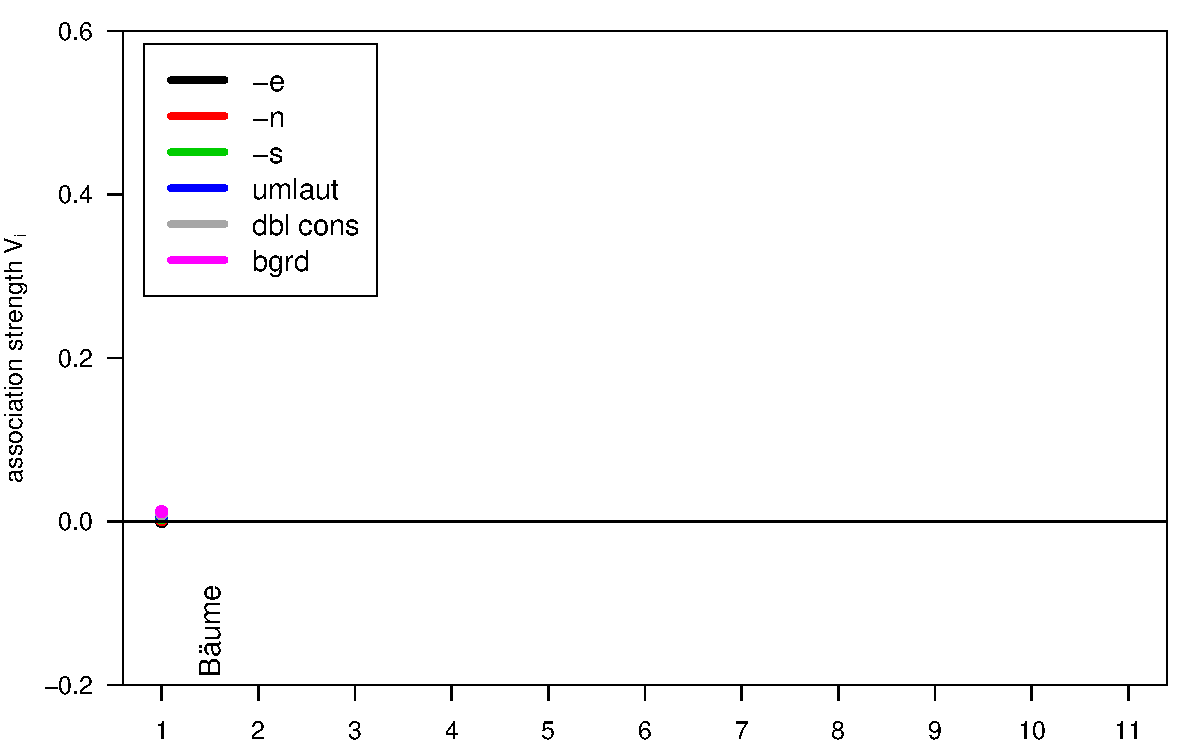
\includegraphics[width=8cm]{img/german_plural_rw_step_1}}%
  \only<beamer:2| handout:0>{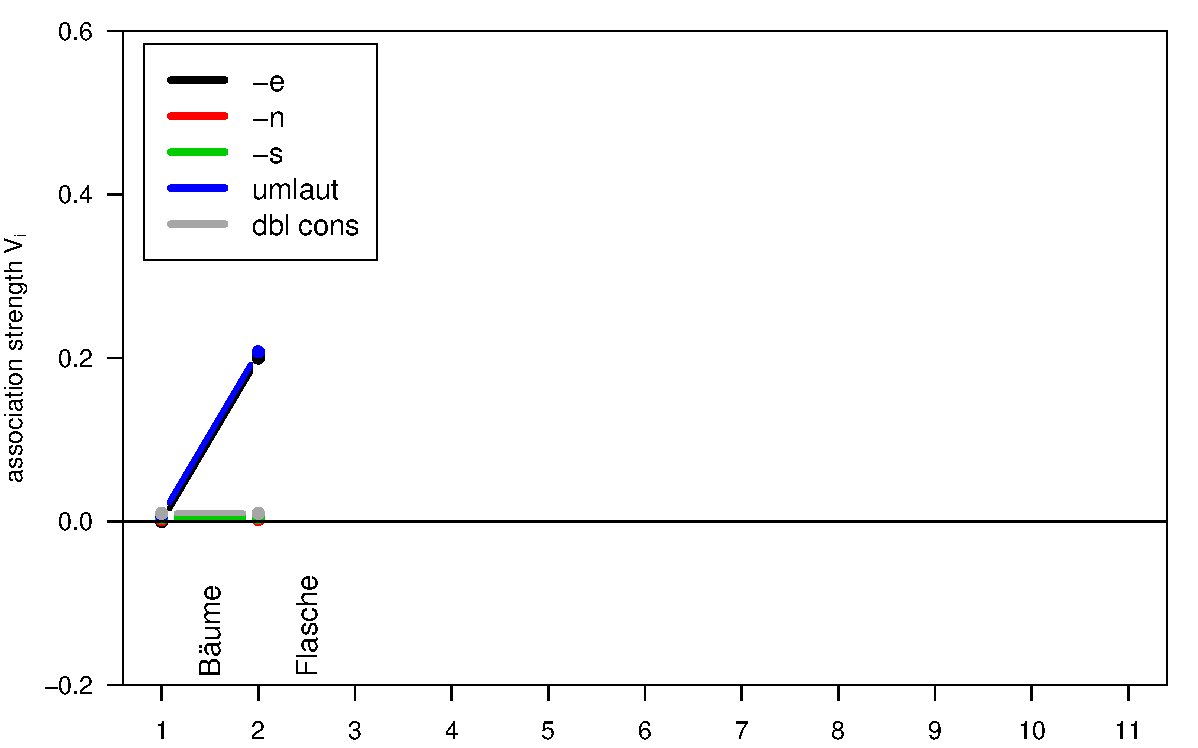
\includegraphics[width=8cm]{img/german_plural_rw_step_2}}%
  \only<beamer:3| handout:0>{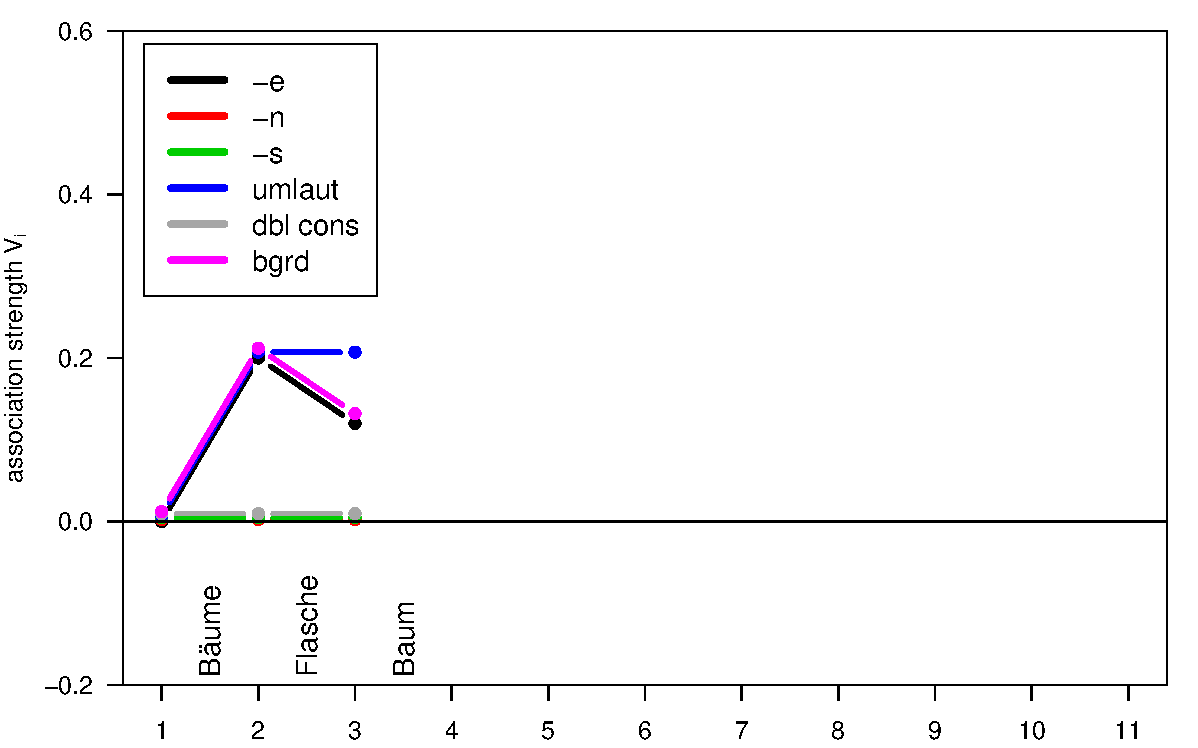
\includegraphics[width=8cm]{img/german_plural_rw_step_3}}%
  \only<beamer:4| handout:0>{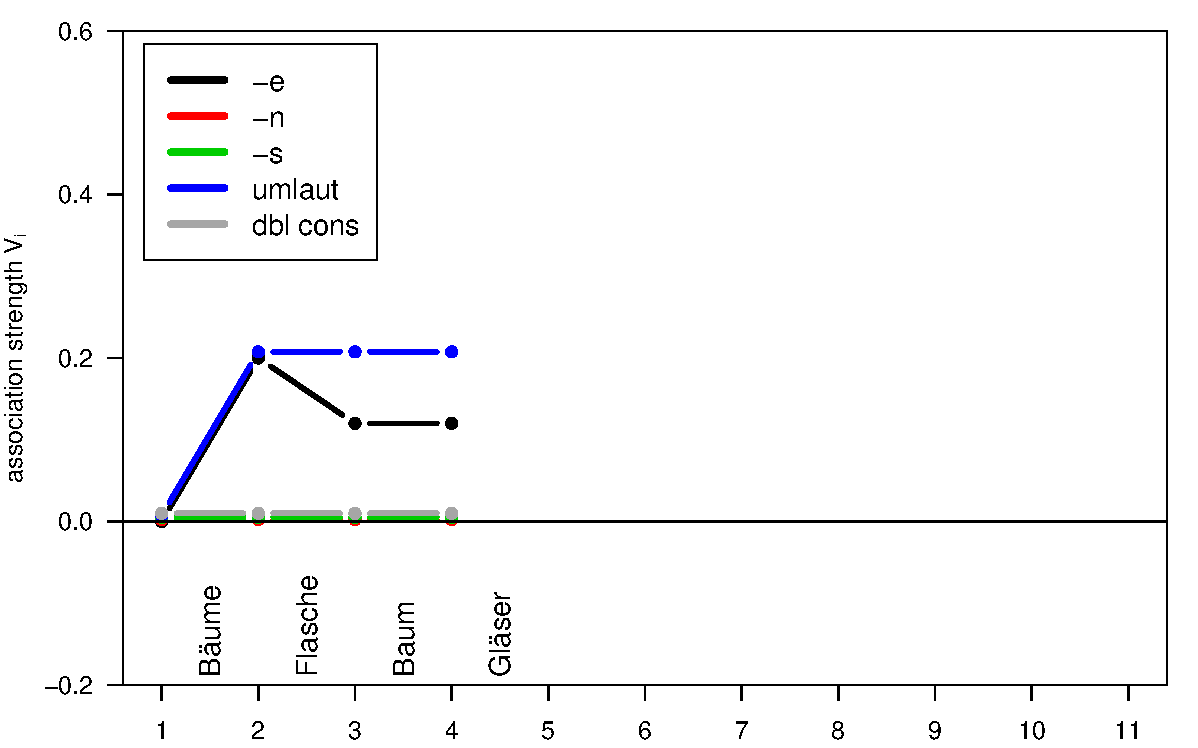
\includegraphics[width=8cm]{img/german_plural_rw_step_4}}%
  \only<beamer:5| handout:0>{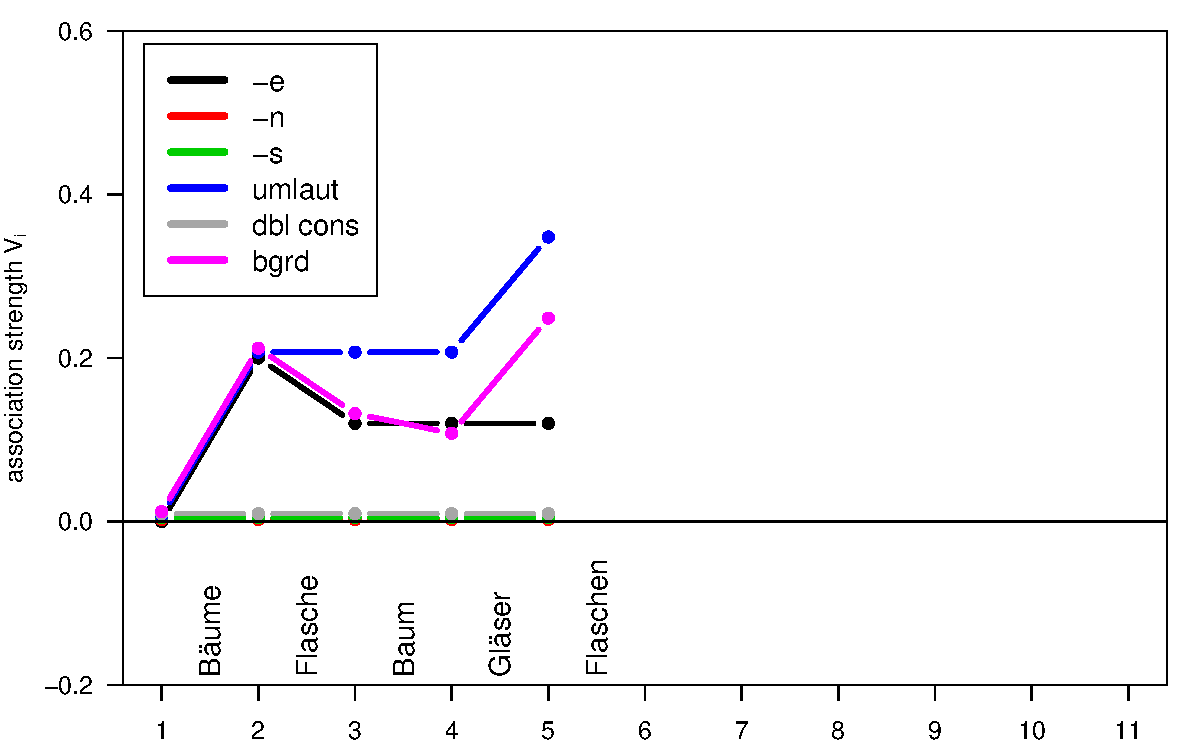
\includegraphics[width=8cm]{img/german_plural_rw_step_5}}%
  \only<beamer:6| handout:0>{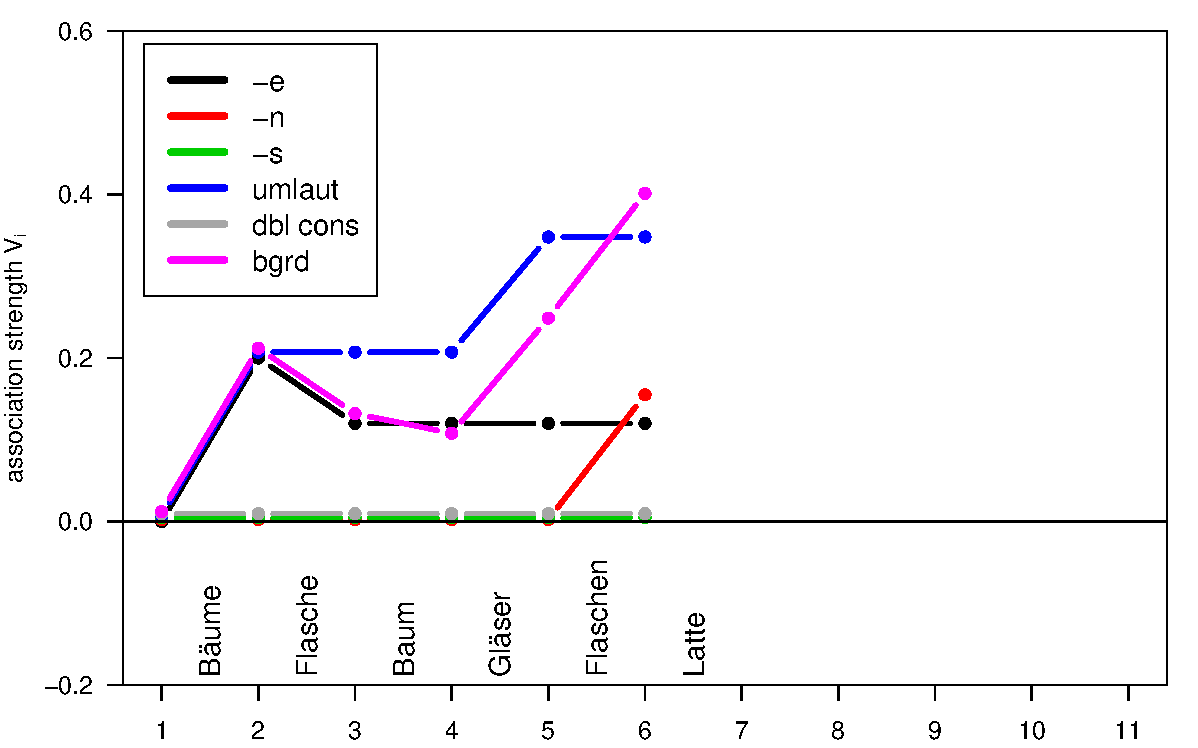
\includegraphics[width=8cm]{img/german_plural_rw_step_6}}%
  \only<beamer:7| handout:0>{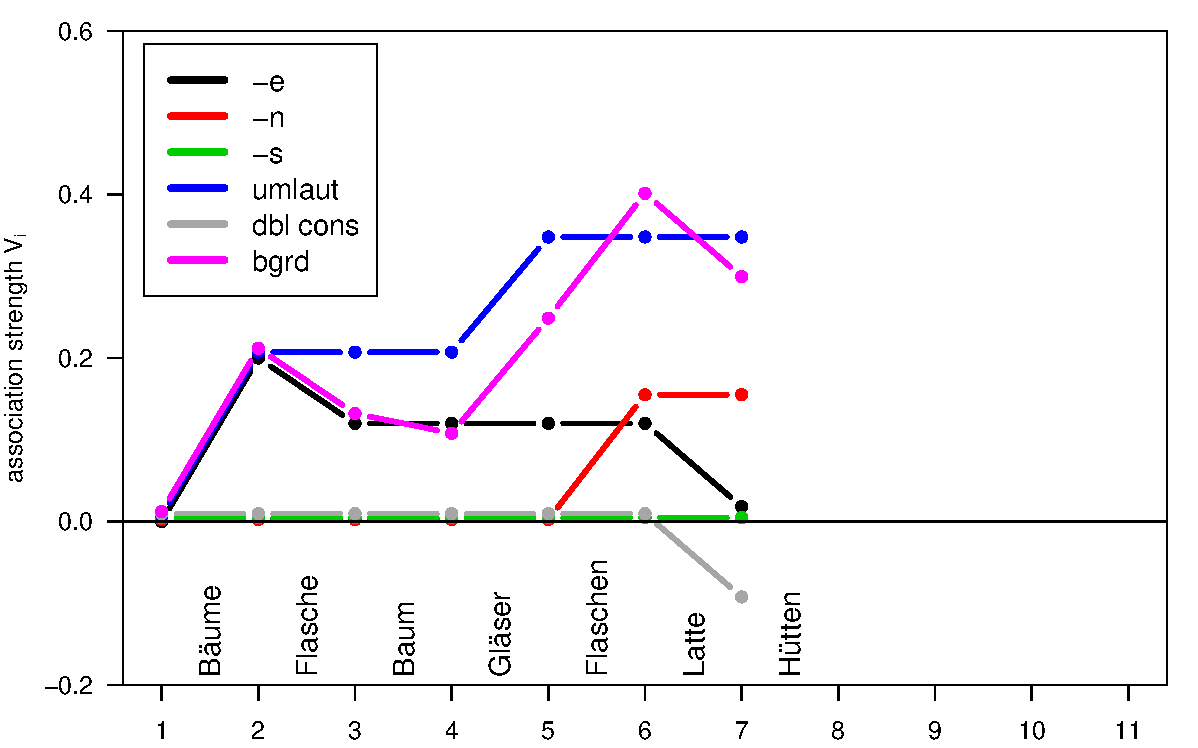
\includegraphics[width=8cm]{img/german_plural_rw_step_7}}%
  \only<beamer:8| handout:0>{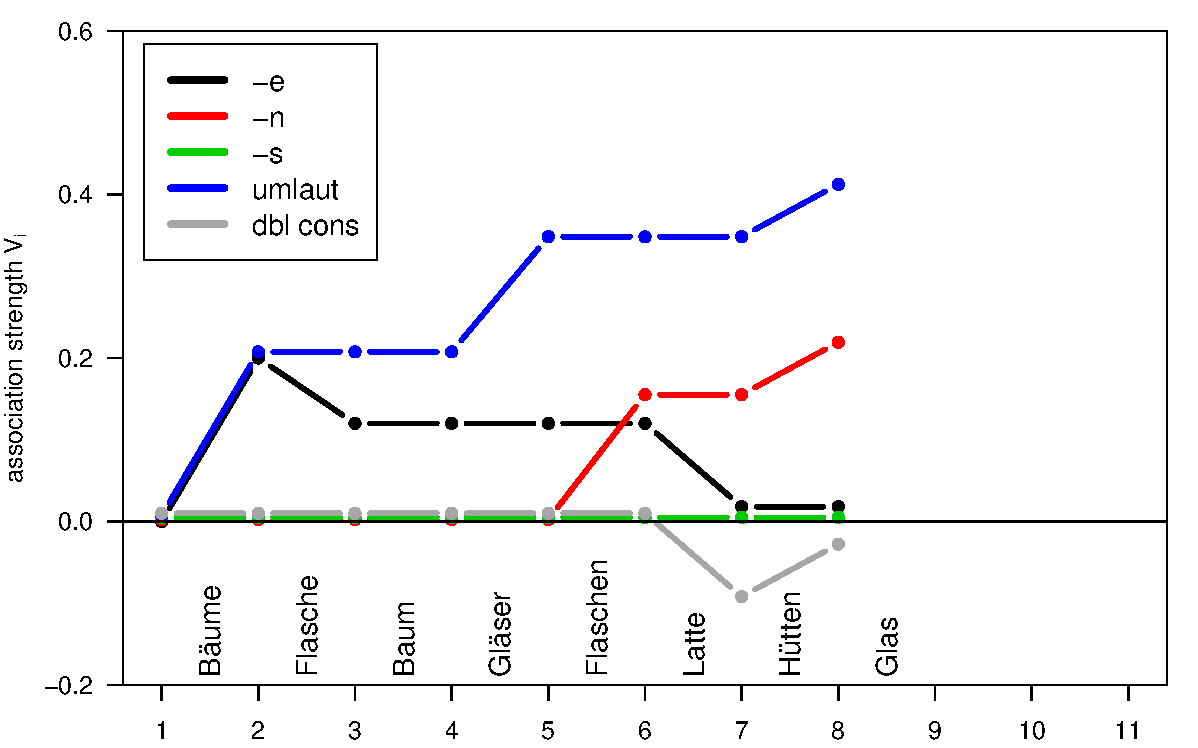
\includegraphics[width=8cm]{img/german_plural_rw_step_8}}%
  \only<beamer:9| handout:0>{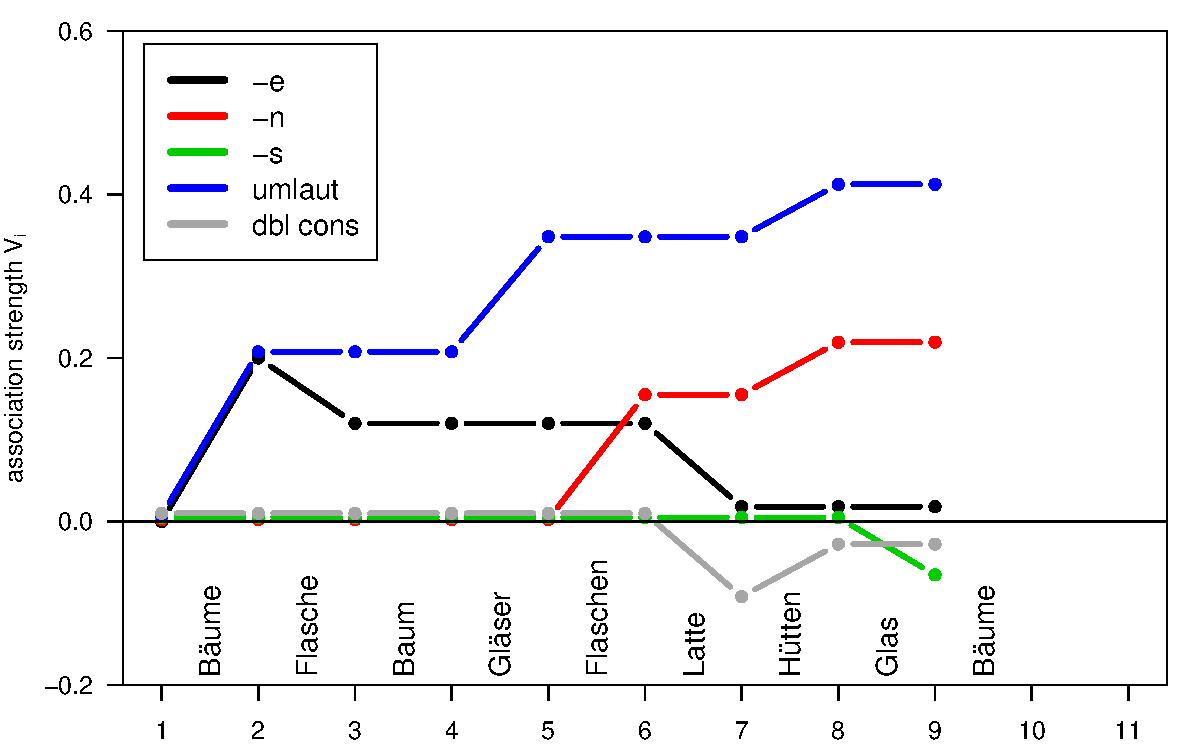
\includegraphics[width=8cm]{img/german_plural_rw_step_9}}%
  \only<beamer:10| handout:1>{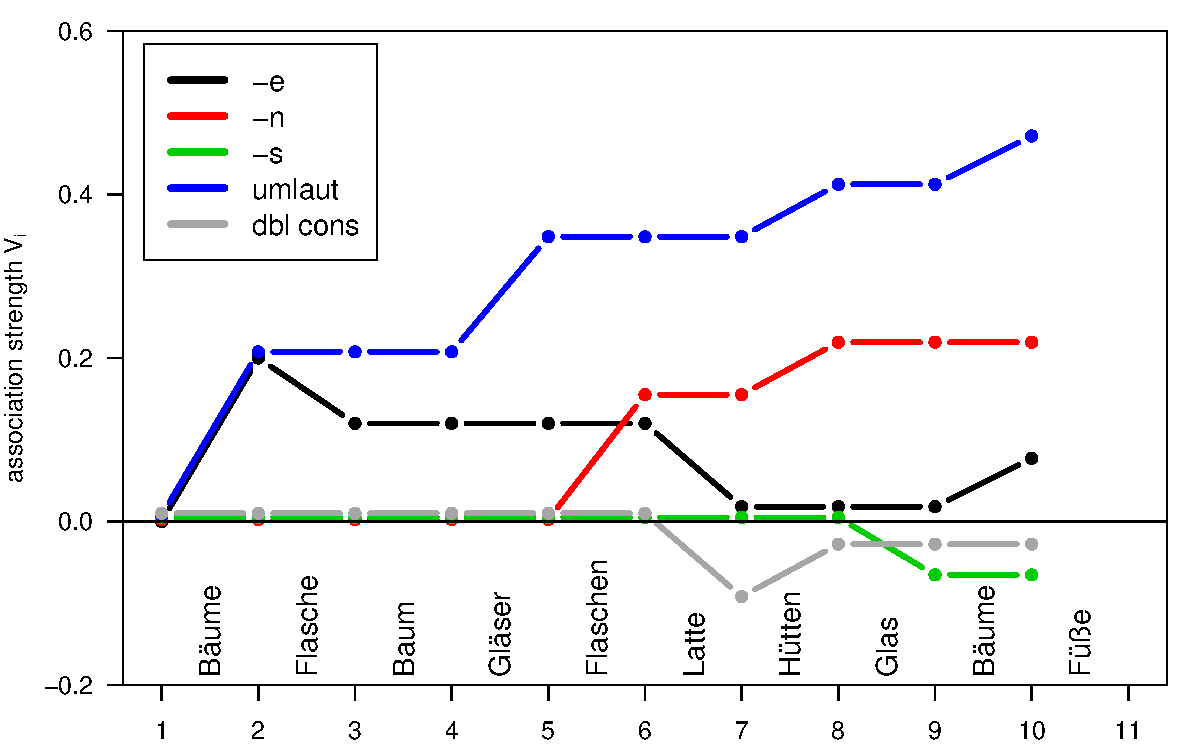
\includegraphics[width=8cm]{img/german_plural_rw_step_10}}%
  \only<beamer:11| handout:0>{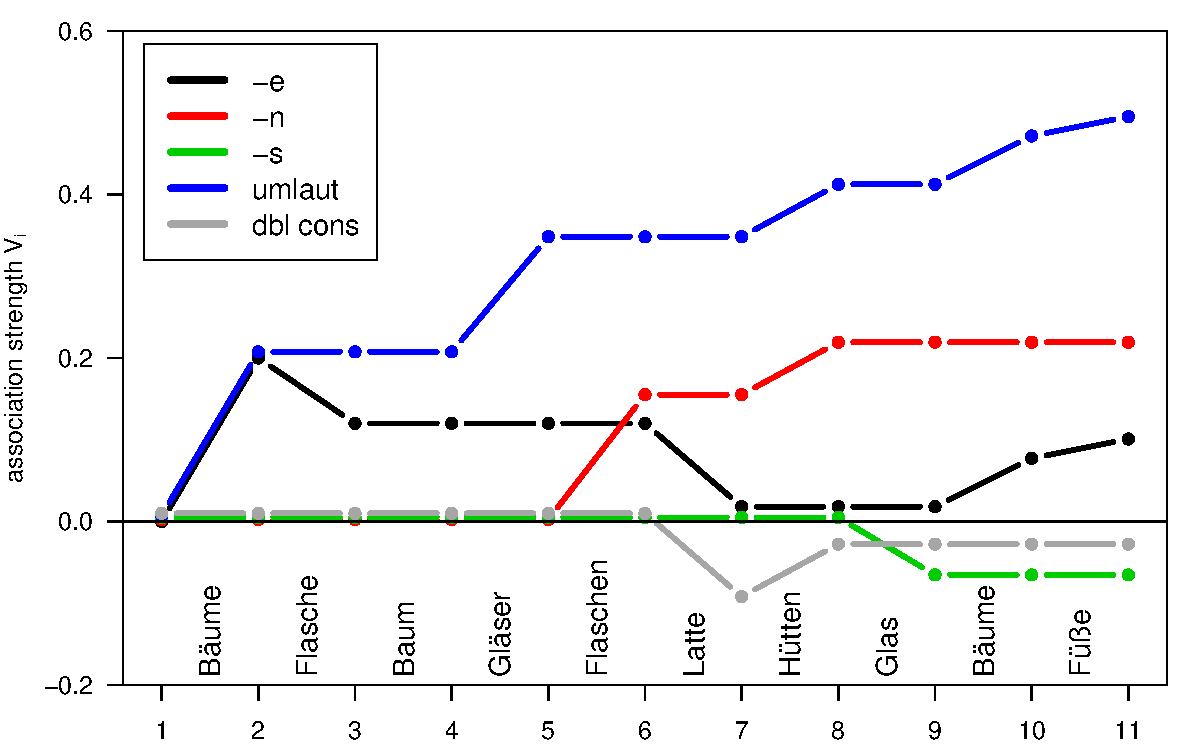
\includegraphics[width=8cm]{img/german_plural_rw_step_11}}%
\end{frame}

\begin{frame}
  \frametitle{A stochastic NDL learner}
  %% \framesubtitle{}

  \begin{itemize}
  \item<1-> A specific event sequence $(\vc[t], o\psupt)$ will only be encountered in controlled experiments
  \item<2-> For applications in corpus linguistics, it is more plausible to assume that events are randomly sampled from a population of \primary{event tokens} $(\vc[k], o\psup{k})$ for $k = 1, \ldots, m$
    \begin{itemize}
    \item[\hand] event types listed repeatedly proportional to their frequency
    \end{itemize}
  \item<3-> I.i.d.\ random variables $\vc[t] \sim \vc$ and $o\psupt\sim o$
    \begin{itemize}
    \item[\hand] distributions of $\vc$ and $o$ determined by population
    \end{itemize}
  \item<3-> NDL can now be trained for arbitrary number of time steps, even if population is small (as in our example)
    \begin{itemize}
    \item study asymptotic behaviour of learners
    \item convergence \so stable ``adult'' state of associations
    \end{itemize}
  \end{itemize}
\end{frame}

\begin{frame}[c]
  \frametitle{A stochastic NDL learner}
  \framesubtitle{Effect of the learning rate $\beta$}

  \centering\ungap[1]
  \only<beamer:1| handout:1>{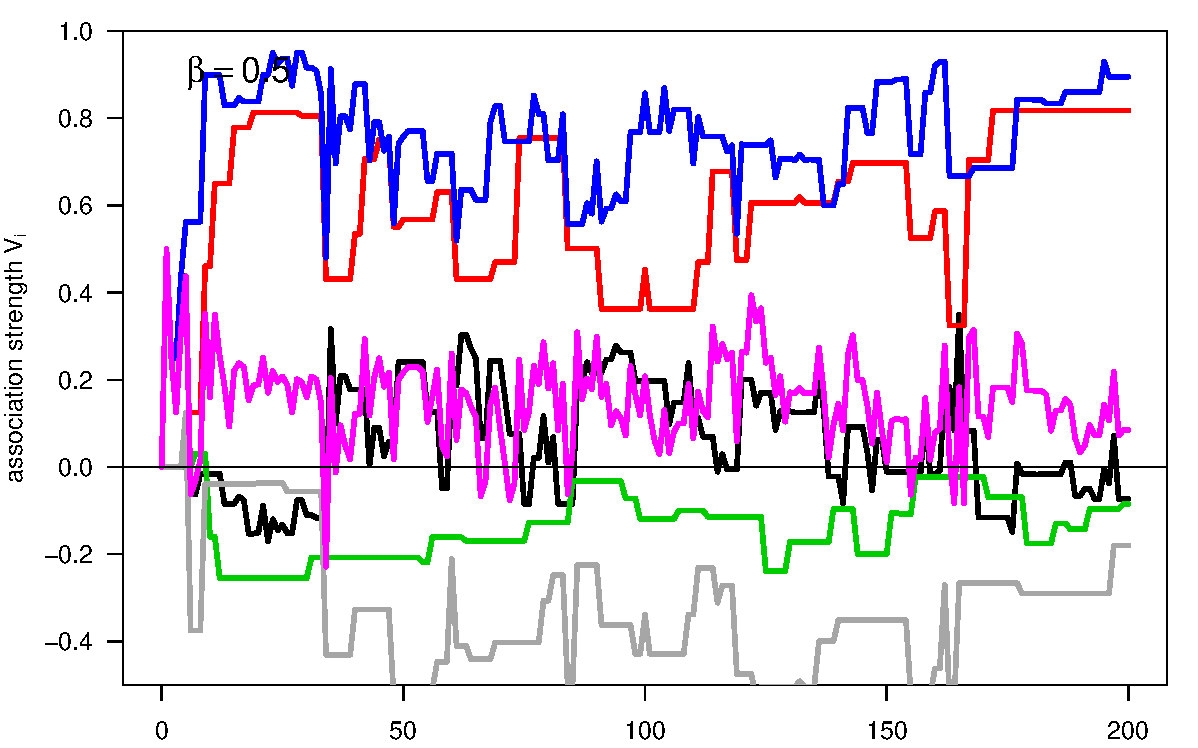
\includegraphics[width=11cm]{img/german_plural_rw_b050_n200}}%
  \only<beamer:2| handout:0>{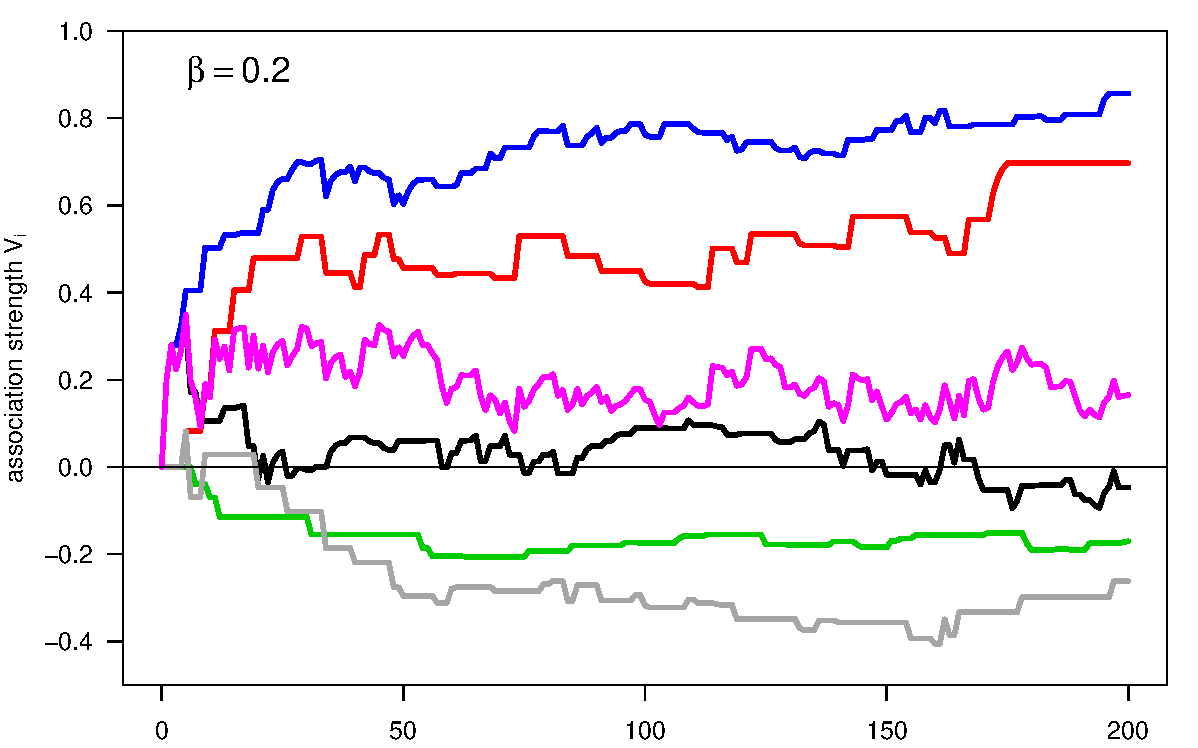
\includegraphics[width=11cm]{img/german_plural_rw_b020_n200}}%
  \only<beamer:3| handout:0>{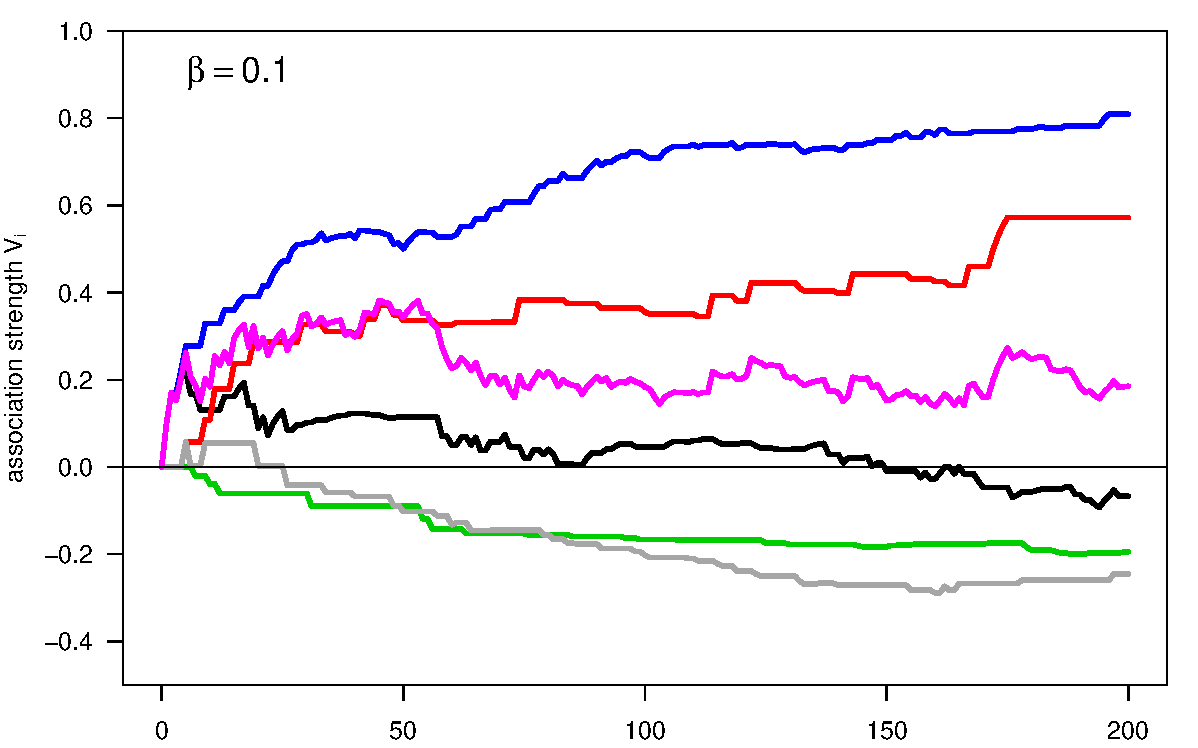
\includegraphics[width=11cm]{img/german_plural_rw_b010_n200}}%
  \only<beamer:4| handout:1>{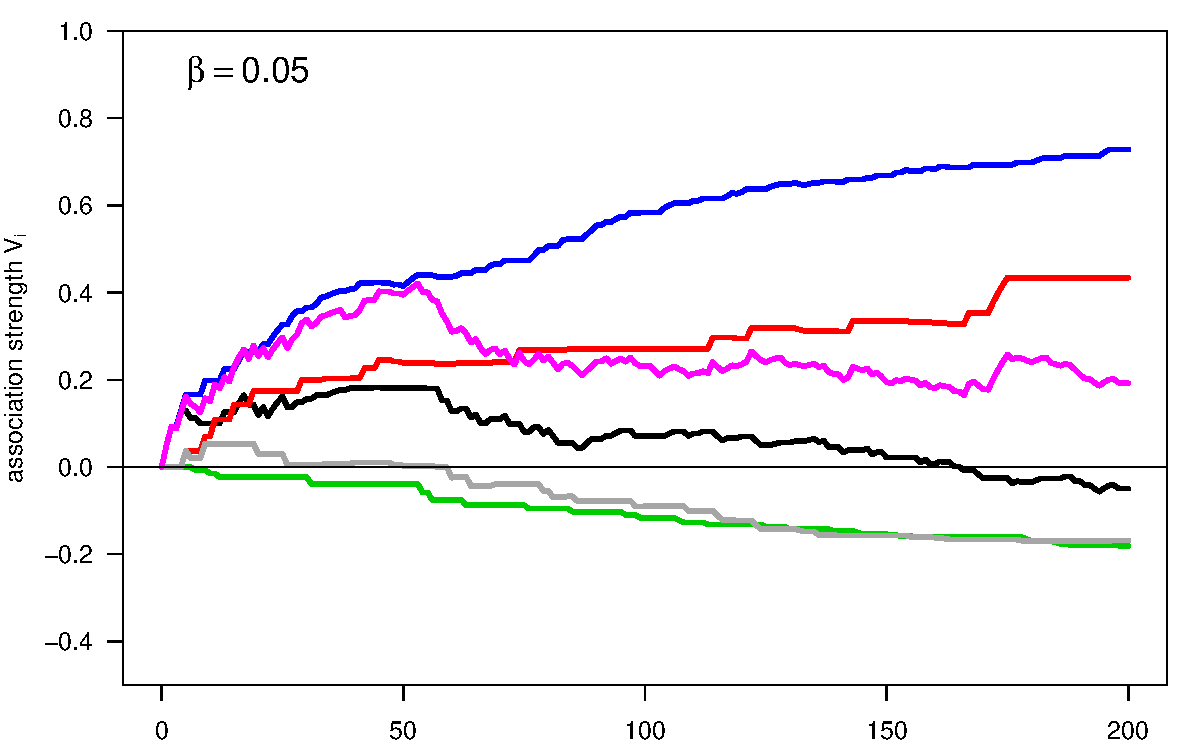
\includegraphics[width=11cm]{img/german_plural_rw_b005_n200}}%
  \only<beamer:5| handout:0>{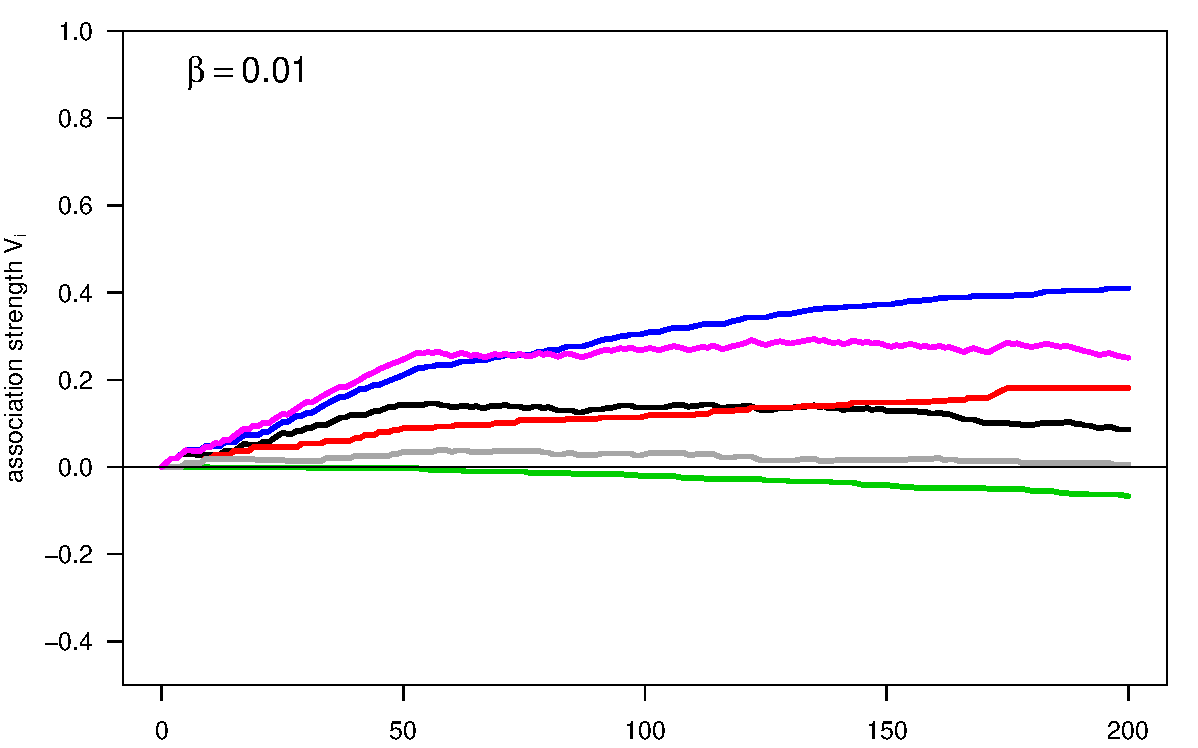
\includegraphics[width=11cm]{img/german_plural_rw_b001_n200}}%
  \only<beamer:6| handout:0>{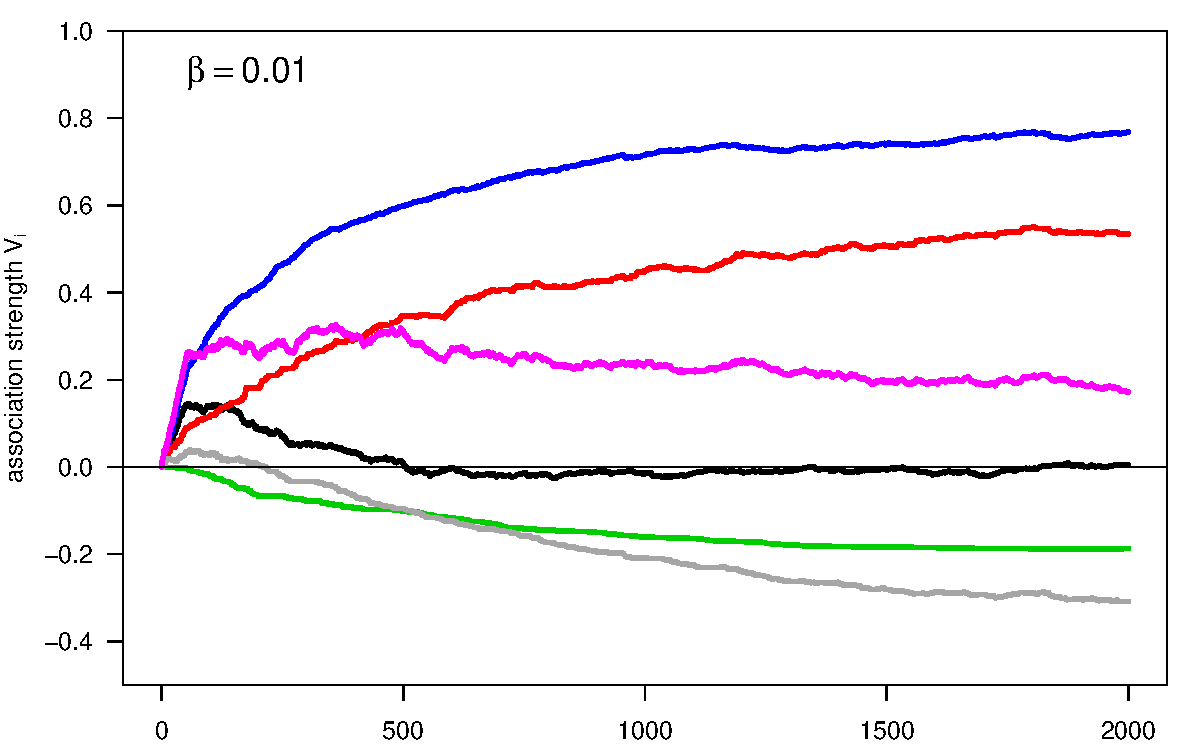
\includegraphics[width=11cm]{img/german_plural_rw_b001_n2000}}%
\end{frame}

%%% Local Variables: 
%%% mode: latex
%%% TeX-master: "../qitl6_evert_arppe"
%%% End: 
